\documentclass[10pt,twocolumn,letterpaper]{article}

\usepackage{cvpr}
\usepackage{times}
\usepackage{epsfig}
\usepackage{graphicx}
\usepackage{amsmath}
\usepackage{amssymb}
% \usepackage{bigfoot}

% Include other packages here, before hyperref.

% If you comment hyperref and then uncomment it, you should delete
% egpaper.aux before re-running latex.  (Or just hit 'q' on the first latex
% run, let it finish, and you should be clear).
\usepackage[breaklinks=true,bookmarks=false]{hyperref}

\cvprfinalcopy % *** Uncomment this line for the final submission

\def\cvprPaperID{****} % *** Enter the CVPR Paper ID here
\def\httilde{\mbox{\tt\raisebox{-.5ex}{\symbol{126}}}}

% Pages are numbered in submission mode, and unnumbered in camera-ready
%\ifcvprfinal\pagestyle{empty}\fi
\setcounter{page}{1}
\begin{document}

%%%%%%%%% TITLE
\title{COMS W4995 Final Report: Automatic Data Augmentation Policy Selection}
\author{Jonathan D. Armstrong\\
{\tt\small jda2160@columbia.edu}
\and
Jesse Galef\\
{\tt\small jbg2160@columbia.edu}
\and
Kyle Matoba\\
{\tt\small km3227@columbia.edu}
}

\maketitle
%\thispagestyle{empty}

%%%%%%%%% ABSTRACT
% \begin{abstract}
% \end{abstract}

% Evaluation metrics for project milestone (20 points)
% Introduction: 2 points
% Related work and references: 2 points
% Problem formulation, technical depth and innovation: 3 points
% Methods, technical depth and innovation, architecture and design: 5 points
% Preliminary results, Github repository, data, code correctness and readability: 8 points

%%%%%%%%% BODY TEXT
\section{Introduction}

In this project, we are working to expand upon the approach used in ``AutoAugment: Learning Augmentation Policies from Data'', \cite{Cubuk2018}. This paper demonstrates success using reinforcement learning to search the parameter space of augmentation policies and identify high quality policies. When this data augmentation is combined with state of the art convolutional neural networks (CNNs), such as \cite{Yamada2018} it achieves state of the art results on the CIFAR 10 dataset,\footnote{\url{https://en.wikipedia.org/wiki/CIFAR-10\#Research\_Papers\_Claiming\_State-of-the-Art\_Results\_on\_CIFAR-10}} and several other canonical test problems in image classification.

\section{Related works}

Data augmentation is indispensable in achieving state of the art performance in image classification. We have seen the best performance achieved by the best architecture wedded to the best data augmentation policy.  One compelling finding to this effect is that \cite{Recht2018} find that out of more than 20 models they entertained, the best-performing model on the CIFAR-10 dataset (\cite{Krizhevsky2009}) was a cutout (\cite{Devries2017}) regularised ``shake-shake'' architecture (\cite{Gastaldi2017}). Cutout is a data augmentation method which appends to the base data set additional occluded images that have had had contiguous regions set to ``zero'' (assuming the data has been normalised around this value). 

Not only was the cutout regularized model best in test-set accuracy, but it was also best on the newly-collected ``CIFAR10.1'' dataset with the smallest drop in accuracy. The other well-performing cutout-regularised model, a wide resnet (\cite{Zagoruyko2016}), whilst beaten by some un-augmented models (though the shake-shake model itself has a straightforward interpretation as data augmentation applied to an representation), both in (test) and out of sample, sees a smaller dropoff between CIFAR 10 test and CIFAR10.1 data sets. 

\section{The significant challenges in achieving the state of the art}

\cite{Cubuk2018} presents a fairly dramatic improvement to the state of the art on a canonical benchmark, essentially by fitting a very computationally demanding model many times to assess the criterion in a discrete optimisation problem. That is to say that this paper demands fairly considerable computation, and the authors, working at Google Brain, clearly have it. 

Using the author's source code, we were able to duplicate their results on CIFAR-10 with several of the smaller architectures, such as a 26 layer ``Shake-Shake`` model of dimension 32 (\cite{Gastaldi2017}) and a Wide Residual Network (\cite{Zagoruyko2016}) with depth 28 and widening factor 10.
For the latter, which required the least computation, a complete fit would have taken about two months on a relatively modern CPU. By running the calculation on the Nvidia K80 GPU offered by Google Colaboratory, we were able to bring the fitting time down to about 27 hours.

\subsection{Hardware Accelerators: GPUs and TPUs}
Getting the computation time down another order of magnitude would be ideal, as it would mean that quick experiments could be done inside of an hour, and the full run, delivering cutting edge results, could be done overnight.

This was in fact possible using TPUs, though unfortunately it was not possible to adapt the \cite{Cubuk2018} author's code to use TPUs, as it was written in an archaic flavour of Tensorflow. In fact, there is an overwhelming consensus online that using TPUs directly from Tensorflow is hazardous, and that using Keras' \texttt|tf.contrib.tpu.keras\_to\_tpu\_model| method was the only mostly-certain way to avoid doing something very dumb. Happily, after much searching, we were able to find a cleanly-coded and correct implementation of the Wide Resnet in Keras. Happily as well, once we had a cleanly-running Keras model, it was straightforward to convert to running on a TPU.

\subsection{A significant aside: The model and success}
We elected to fit a relatively simpler and faster architecture, the Wide Residual Network (\cite{Zagoruyko2016}) -- our experiments showed that this model fit between 10 and 100 times more quickly than the best-performing models, so even on a TPU following best practice and under totally ideal conditions, it would not have been possible to do a fit of these models more than once or twice before the deadline. The author of \cite{Gastaldi2017} further bemoans the considerable computational challenges he faced in achieving his results as an individual without substantial computational resources.

Since empirically, the only thing faster than a TPU would be a cluster of TPUs or a massive cluster of GPUs, we can be confident that it would not have been possible to fit this model short of thousands of dollars of google cloud compute credit, or else some \emph{very} cutting-edge optimisations. In our researsh, most of the serious optimsations are coded in Pytorch (precluding the use of TPUs), and use (wide) resnets anyway. For one very cool flavour of this, see the ranking at \url{https://dawn.cs.stanford.edu/benchmark/#cifar10}) of the \cite{Coleman2017} DAWNBench project.

Based on the comparison of autoaugmented and more simply augmented models presented in \cite{Cubuk2018}, we think that our results should transfer straightforwardly to architectures that perform better un-augmented. This is because the best results seem to be achieved pretty straightforwardly by stacking the best data augmentation schemes atop the best un-augmented architectures -- a separability essentially making totally state of the art results achievable to anyone with sufficient computational wherewithal to fit them.

% As mentioned, we achieve state of the art results in a particular format: the best classification performance from an off-the-shelf model that could be run for free by someone with a google account overnight.

\subsection{Google Colab and Drive}
An embarassing quantity of effort went into adapting the Colaboratory platform for non-interactive use -- making it more robust to server-side outages and persisting data and results across sessions. This entailed a fairly deep delve into the programmatic control over Colaboratory and Jupyter Notebooks, as well as the better-documented Google Drive API (besides experiments with Dropbox and others). By the end, we had crafted a fairly sophisticated checkpointing and recovery process for the efficient and effective use of Google Colaboratory backed by Google Drive. 

Whilst this time was essentially wasted in the sense that we learned nothing of academic or conceptual import, it was surely not wasted in a more general and perhaps more important issue: it let us achieve world class results without access to hundreds of petaflops of computation. This concern, that the best results may only in future be achievable to those with the financial resources has featured in a recent Columbia Colloquim by John Henessy and has been a topic of considerable interest at the NeurIPS 2018 Conference. % and its attendant press coverage.\footnote{Cf. \url{https://www.bloomberg.com/news/articles/2018-11-30/visa-issues-cast-shadow-on-canada-s-moment-in-the-ai-spotlight}}

\section{Results}

As an aside, one should note that 100\% accuracy sould seem to not even be achievable -- there are mistakes even in the CIFAR data there are misclassifications!  \footnote{To see this, load the test data, e.g. with \texttt{\_, (xtest, ytest) = keras.datasets.cifar10.load\_data()}, then examine the 2406th entry, e.g. \texttt{plt.imshow(xtest[2405, :, :, :])} -- pretty evidently a frog, but labelled as a cat!}

\subsection{Observations}

Another interesting phenomenon we noticed (we think!) with the Wide Resnet is the ``compression'' described by the professor in class, following \cite{Shwartz-Ziv2017}. The training and validation error tend to rise rapidly in only a few dozen epochs, but the generalisation error is terrible if one stops as soon as the errors begin flattening out (so bad, in fact, that we thought we had made a mistake). I found the mutual-information-based presentation interesting and subtle, but observing it in practice really made me realise how interesting and counterintuitive the result really is. I think that one of the most useful takeaways from this course is that the ``early stopping $\implies$ regularisation $\implies$ better generalisation error`` chain of implications is sloppy thinking and often incorrect in very relevant situations!


\subsection{Reduced AutoAugment}
Each policy of data augmentation requires selecting 10 operations, each with one of 16 transformations, 11 discrete probabilities of application, and 10 magnitudes.  The resulting action space has approximately $2.9 \times 10^{31}$ possible actions, making a policy-gradient reinforcement learning approach preferable.One challenge in vanilla policy gradient methods is finding a way to update weights without moving too far from the current policy. Several surrogate loss functions have been designed to encourage or enforce smaller steps, including Trust Region Policy Optimization (TRPO) and now Proximal Policy Optimization (PPO). AutoAugment uses a variant called PPO-Clip, developed by OpenAI \cite{Schulman2017}. PPO-Clip implements a surrogate loss function that includes a clipped term for how much more or less likely the sampled action trajectory would be under the new policy. The AutoAugment controller model samples and scores a batch of policies before using stochastic gradient descent to optimize for this loss function.

\begin{figure}[h]		
\begin{center}
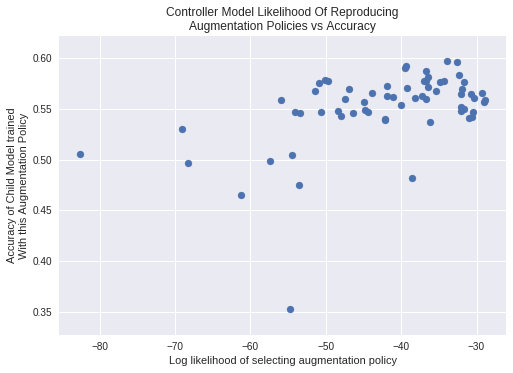
\includegraphics[width=0.5\textwidth]{ReducedAutoAugment.png}
\end{center}
\caption{Accuracy vs. Log-Likelihood}
\label{fig:RAA}
\end{figure}
		We implemented a controller model that uses PPO-Clip reinforcement learning. For each training epoch, it produces a batch of data augmentation policies, trains basic 'child models' with them, then uses their validation accuracy as a reward signal. To verify that the controller model was correctly learning to produce better policies, we trained it for 8 epochs - a relatively small number, but enough to check that the algorithm was correct. We found a correlation of .49 between the log likelihood of producing a policy and the quality of that policy, indicating that the model was improving (see figure~\ref{fig:RAA}).

\subsection{Naive Analysis}
The results of this analysis strongly depend on the validity of comparing different test accuracies. Additionally, it is desirable to get meaningful results quickly. In order to manage these requirement we used the following approaches

\begin{enumerate}
\item We removed dependency on the random initialization of weights by starting with a partially trained ``base`` model. Each policy is then trained using a copy of this base.
\item We must be sure each model has been fully trained. We acheive this (and reduced training time) by removing the model's dropout layers so that the validation loss achieves a prominent minimum. We then configure the training to hold the weights corresponding to the best validation accuracy.
\item To further reduce training time, we follow the lead of the AutoAgument authors and trained on a reduced version of the CIFAR-10 dataset consisting of 4000 images randomly selected from the training set.
\end{enumerate}

Using this scheme, our initial results appear in the table below.



With the setup described above, we trained the base model against several different policies and achieved the results summarize in the table below.

		\begin{table}[h]
			\begin{tabular}{l|l}
				\hline
				Policy  						&Test Accuracy (\%)   \\ \hline
				Baseline (No Augmentation)  	&49.6 \\
				Single Transform				&46.6 to 53.1 \\
				AutoAugment 					&53.3 \\ 
				AutoAugment Random				&53.1 \\	
				AutoAugment Subset Random 		&55.1 \\
				Category Targeted Policies   	&50.0 to 54.7 \\
				Best Transforms as Subpolicy 	&55.5
			\end{tabular}
			\caption{Test accuracies with different policies}
		\end{table}
	
\section{Augmentation Policy Architecture}
We will use the following definitions (generalized from the AutoAugment Procedure):

\begin{enumerate}

\item[] \textbf{Transform}: a single transform that can be applied to an image. This transform is parameterized by the a level (e.g. magnitude of the transform, in the integer range $0,1 \cdots, 10$), and the probability of applying the transform. The probability is quantized, taking values in the range $\{0.0, 0.1, 0.2, \cdots, 0.9, 1.0\}$; the level is both quantized and normalized to a predefined range, for example the ``rotate`` transform's maximum magnitude of $30$ degrees is the upper bound corresponding to a level of 10. Note that for many transforms such as ``auto\_contrast`` and ``flip\_lr`` ignore the level parameter.
\item[] \textbf{Sub-policy}: a sequence of transforms that are applied in series to an image
\item[] \textbf{Policy}: a set of Sub-Policies. For each mini-batch, a subpolicy is randomly chosen (uniformly) and applied.
\end{enumerate}

The set of twenty transforms considered exactly correspond to those of the AutoAugment transforms: \textit{flip\_lr}, \textit{flip\_ud}, \textit{auto\_contrast}, \textit{equalize}, \textit{invert}, \textit{rotate}, \textit{posterize}, \textit{crop}, \textit{solarize}, \textit{color}, \textit{contrast}, \textit{brightness}, \textit{sharpness}, \textit{shear\_x}, \textit{share\_y}, \textit{translate\_x}, \textit{translate\_y}, \textit{cutout}, \textit{blur}, and \textit{smooth}. 

The AutoAugment policy architecture consists of five sub-policies, each built from two transforms. On completion, a final super-policy is generated by concatenating sub-policies from the five best policies to create a policy with $25$ sub-policies.

\subsection{}

To establish a \textbf{Baseline} policy, we first completed training with no data augmentation. Then, for each of the 20 transforms defined in \textit{AutoAugment}, we tested a policy built purely from that one transform (fixed probability $0.5$ and level $5$); these are labeled collectively as \textbf{Single Transform}. Many canonical transforms for CIFAR-10 made it to the top of the list including \textit{flip\_lr} (mirror) and \textit{rotate} with test accuracies of 53.1\% and 50.7\% respectively. On par with \textit{rotate} is also the less common transform \textit{solarize} with a test accuracy of 50.9\%. The worst performer here was \textit{blur} with a test accuracy of 46.6\%; considering the low resolution of the images this comes as no surprise.

In addition to testing the \textit{AutoAugment} policy, we developed two additional variants to explore the possibility that the AutoAugment procedure is over-engineered. First, \textbf{AutoAugment Random} is identical in structure to the original AutoAugment policy, but the transforms, probabilities, and levels are set randomly. Second, \textbf{AutoAugment Subset Random} also uses identical structure but draws from the subset of transforms that individually outperformed the \textbf{Baseline} policy by once percent (\textit{flip\_lr}, \textit{translate\_y}, \textit{translate\_x}, \textit{shear\_y}, \textit{solarize}, and \textit{rotate}). The most significant result here is that we were able to comfortably beat the performance of the \textbf{AutoAugment} policy by $1.7\%$ with a randomly generated policy (informed by our analysis results).

Analysis of the category-level accuracies demonstrated significant differences between \textbf{Baseline} and \textbf{Single Transform} policies. For example, \textit{translate\_y} increased accuracy for the ``frog`` category by more than $37\%$. Using the test accuracy differences for each transform, we explored different algorithmic approaches to creating category targeted policies (with varying architecture) and achieved test accuracies from $50.0$ up to $54.7$. The architectures on the lower end of performance combined the best transforms for each category and mixed them into sub-policies; these policies topped out at $50.0\%$ test accuracy and were not able to outperform the best single transform (\textit{flip\_lr} at $53.1\%$). The architectures on the high end of performance use one transform for each sub-policy with identity masking for categories where the transform performed poorly. With this approach, we observed that test accuracy increased as we eased the identity masking threshold for each category. Ironically, this approach converged to the \textbf{Best Transforms as Subpolicy} policy which no longer differentiates between image categories! This policy was algorithmically generated by selecting the transforms that improved the baseline test accuracy by one percent and then used that transform as a sub-policy. This approach mimicked the \textit{AutoAugment Subset Random} policy in the transforms considered, but used a much simpler policy architecture with fixed levels and probability ($5$ and $0.5$ respectively). This policy obtained the best test accuracy, $55.5\%$.

To further verify the effectiveness of the \textbf{Best Transforms as Subpolicy} policy, we retested with the full CIFAR-10 training dataset (with 10\% reserved for validation) and restored the dropout layers to the model. Note that each model was trained from scratch without using a shared partially-trained base model. The following table contains the results of this test.

\begin{table}[h]
    \begin{tabular}{l|l}
        \hline
        Policy                          &Test Accuracy (\%)   \\ \hline
        Baseline (No Augmentation)      &80.5 \\
        AutoAugment                     &82.3 \\
        Best Transforms as Subpolicy    &84.1 \\
    \end{tabular}
    \caption{Full dataset, model; test accuracies with different policies}
\end{table}

With \textbf{Best Transforms as Subpolicy} at the top again, these results provide evidence that it may be possible to outperform AutoAugment with a much simpler procedure. The natural next step now is to use this augmentation policy to train world-class models and see if we can outperform AutoAugment!


Note that this approach outperforms the original \textbf{AutoAugment} policy event though the transform parameter space is much less dynamic; probabilities are fixed at $0.5\%$ and the level are fixed at $5\%$.

\section{Link to Github}
	%Currently the work is spread across a few repos, as well as Google Colab notebooks. We will work to consolidate things into a single, cleanly-runnable shape as we approach conclusion.

	\begin{itemize}
	\item \url{https://github.com/kylematoba/deeplearning-project}
	\item \url{https://github.com/kylematoba/models}
	%\item %\url{https://colab.research.google.com/drive/1qV3vCsjnEcm5a8nRpN40n4qgVKKBzBkd#scrollTo=uiht7wpPPPCP} (also checked into the \texttt{deeplearning-project} repo above)
	%\item \url{https://colab.research.google.com/drive/13GpO9tSqLxflZ9Z2B6RkWMVzfcemW2v7}
	\end{itemize}

% Note that we've not made the repo public, but we have permissioned \texttt{id2305@columbia.edu}, \texttt{id2303@columbia.edu}, \texttt{}

\nocite{Torralba2008}
{\small
\bibliographystyle{ieee}
\bibliography{../biblio}
}

\end{document}

